% -*- coding: utf-8 -*-
% !TEX root = ../main.tex

\subsection{Télécom SudParis}\label{ssec:introduction_nom_entreprise}

% TODO Présenter l'entreprise et ses objectifs
Télécom SudParis est une grande école d'ingénieurs du numérique localisée à Évry, en France, et certifiée par la Commission des Titres d'Ingénieurs.\
Celle-ci fait partie de l'Institut Mines-Télécom et est membre de l'Institut Polytechnique de Paris.\\
L'école compte environ 1000 étudiants et plus d'une centaine de doctorants.\
Les thématiques étudiées tournent autour des Mathématiques Appliquées, de l'Informatique, des Réseaux, du Signal, et de la Physique.\\
L'équipe pédagogique est composée de plus d'une centaine d'enseignants chercheurs dont les travaux portent sur des thématiques comme les
réseaux complexes, le big data, l'IA, le cloud, l'Internet des objets ou encore la cybersécurité.\

% Exemple pour pour une image
% Rappel | Formats acceptés par \includegraphics (défaut) : png, jpg, pdf...
\begin{figure}[!h]
    \centering
    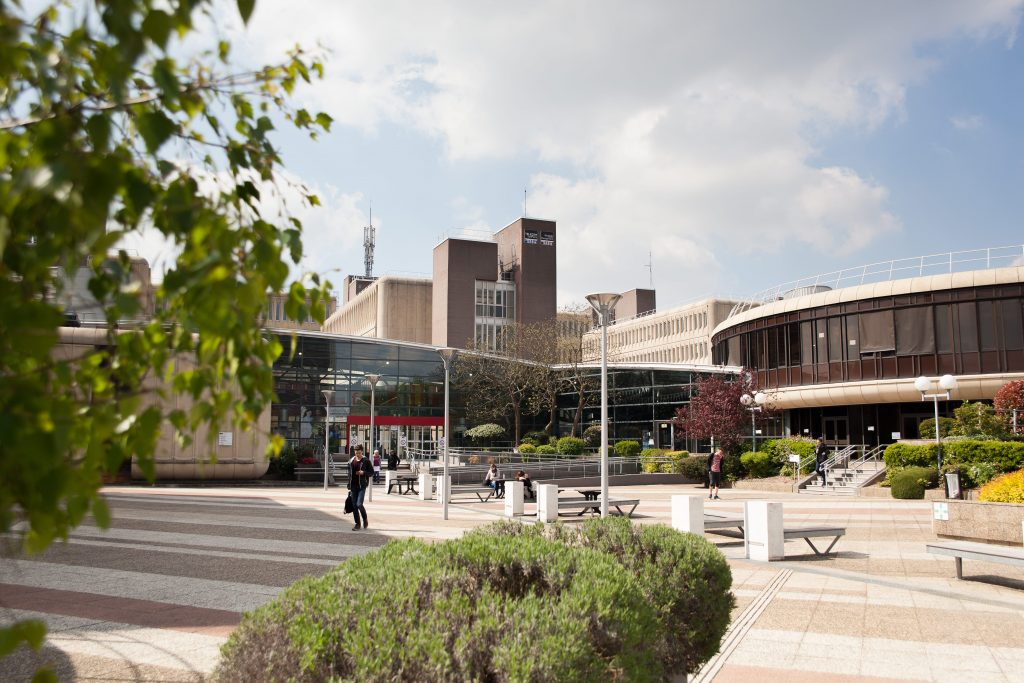
\includegraphics[width=0.7\textwidth]{img/campus_tsp.jpg}
    \caption{Photo du site}
    \label{fig:photo_site}
\end{figure}

%%%%%%%%%
%%%%%%%%%
%%%%%%%%%
%%%%%%%%%

\subsection{Service d'accueil}\label{ssec:introduction_service_accueil}

Ce stage a été encadré par \verb!François TRAHAY!, enseignant à \verb!Télécom SudParis! et chercheur au sein du laboratoire de recherche \verb!SAMOVAR! (Serivces répartis,\
Architectures, Modélisation, Validation, Administration des Réseux). Ce laboratoire accueille également quelques enseignants-chercheurs de l'\verb!ensIIE!, comme \verb!Valentin HONORÉ! qui a notamment co-encadré ce stage.\
Leurs travaux de recherche récents sont orientés vers l'analyse des performances dans le domaine du HPC (High Performance Computing).\
De plus, ils font partie de l'équipe \verb!BENAGIL! qui étudie la conception de systèmes distribués plus efficaces et plus sûrs en se focalisant sur leurs composants essentiels.

% TODO Présenter service/département de travail et son rôle dans entreprise
% On pourra aussi préciser le matériel à notre disposition pour mener notre stage

%%%%%%%%%
%%%%%%%%%
%%%%%%%%%
%%%%%%%%%

\subsection{Contexte et problématique}\label{ssec:introduction_contexte_problematique}

Le PEPR NumPEx est un projet de recherche qui a pour objectif l'élaboration de la pile logicielle de la future machine exascale française, Alice Recoque. L'équipe dirigée par \verb!François TRAHAY!
fait partie du sous-projet Exa-SofT qui cherche à fournir les logiciels et outils de support aux applications. Plus précisément, l'équipe a pour objectif de fournir des outils pour l'analyse des performances
adaptés au passage à l'échelle exascale. \\
Afin de réaliser une analyse fine des performances, on utilise les traces d'exécution qui constituent une représentation de tous les évènements ayant lieu lors de l'exécution d'un programme.
Actuellement, il existe des formats de trace tels que \verb!OTF2! qui stockent les données sans une structure permettant de factoriser les évènements identiques ou bien une analyse rapide sans charger toutes les données. 
Afin de capturer tous les évènements d'un programme on utilise un outil de traçage, \verb!EZTrace! qui a été notamment 
développé par \verb!François TRAHAY!.
\\Ainsi, le travail de recherche est centré sur le développement d'un nouveau format de trace d'excution, \verb!PALLAS!, qui doit permettre de tracer des programmes HPC s'exécutant à très large échelle
(plus de 4096 threads).\\
\verb!PALLAS! est un format de trace générique (supportant plusieurs outils tels que \verb!OpenMP!, \verb!MPI!, \verb!CUDA!, ...) permettant de factoriser de manière structurée les différents évènements 
regroupés en boucles et en séquences. La structure de ces traces permet une analyse post-mortem efficace, avec notamment des outils déjà mis en place comme une matrice
de contention et de communication.




%%%%%%%%%
%%%%%%%%%
%%%%%%%%%
%%%%%%%%%

\subsection{Objectifs du stage}\label{ssec:introduction_objectifs}

Les objectifs de ce stage sont de réaliser une analyse précise des performances de certains aspects de \verb!PALLAS!. Dans un premier temps une analyse de l'application de \verb!pallas_print! permettant
l'affichage de toute la trace a été réalisée, puis de manière plus globale l'étude de l'overhead induit par \verb!PALLAS! et l'analyse des processus de compression et d'écriture de la trace sur les disques (temps d'exécution mais 
également évaluation de la perte d'information causée par la compression). 


%%%%%%%%%
%%%%%%%%%
%%%%%%%%%
%%%%%%%%%

\subsection{Contributions principales}\label{ssec:introduction_contributions}
À travers ce stage j'ai pu proposer une étude approfondie de différents aspects de la librairie \verb!PALLAS!, avec notamment un travail autour des fonctions d'écriture et de compression
de la trace.
Afin de réaliser cela, j'ai mis un place un certain nombre de scripts \verb!bash! pour mettre en place en exécuter les différentes applications et benchmarks ainsi que des 
scripts \verb!python! afin de réaliser les différents graphiques présentés dans la suite de ce rapport.
